\documentclass{standalone}
%
\usepackage{tikz}
%
\usepackage{tkz-euclide}
\usetkzobj{all}
%
\usepackage{xcolor}
\definecolor{space}{HTML}{1F2C4E}
\definecolor{earth}{HTML}{0089FA}
\definecolor{dida}{HTML}{FFDE00}
\definecolor{title}{HTML}{FBA706}
\definecolor{moon}{HTML}{AFAFAF}
\definecolor{craterm}{HTML}{616060}
%
\usepackage{fontspec}
\setmainfont{Open Dyslexic}
%
\title{L'eclissi di Eddington}
\begin{document}
	\tikzset{
		partial ellipse/.style args = {#1:#2:#3}{insert path={+ (#1:#3) arc (#1:#2:#3)}},
	}
	\begin{tikzpicture}
		\draw [use as bounding box] (0,15.5) -| (30,15.5) |- (30,-97) -| (0,-97);
		%title
		\draw [black,ultra thick,fill=title] (-1,7) rectangle (31,15);
		\node (example-textwidth-2) [right, align=center, text width=30cm, color=black, font=\fontsize{90pt}{91pt}\selectfont] at (0,11) {L'eclissi di Eddington};
		% island
		\begin{scope}[shift={(0,-8)}]
			\node at (15,0) {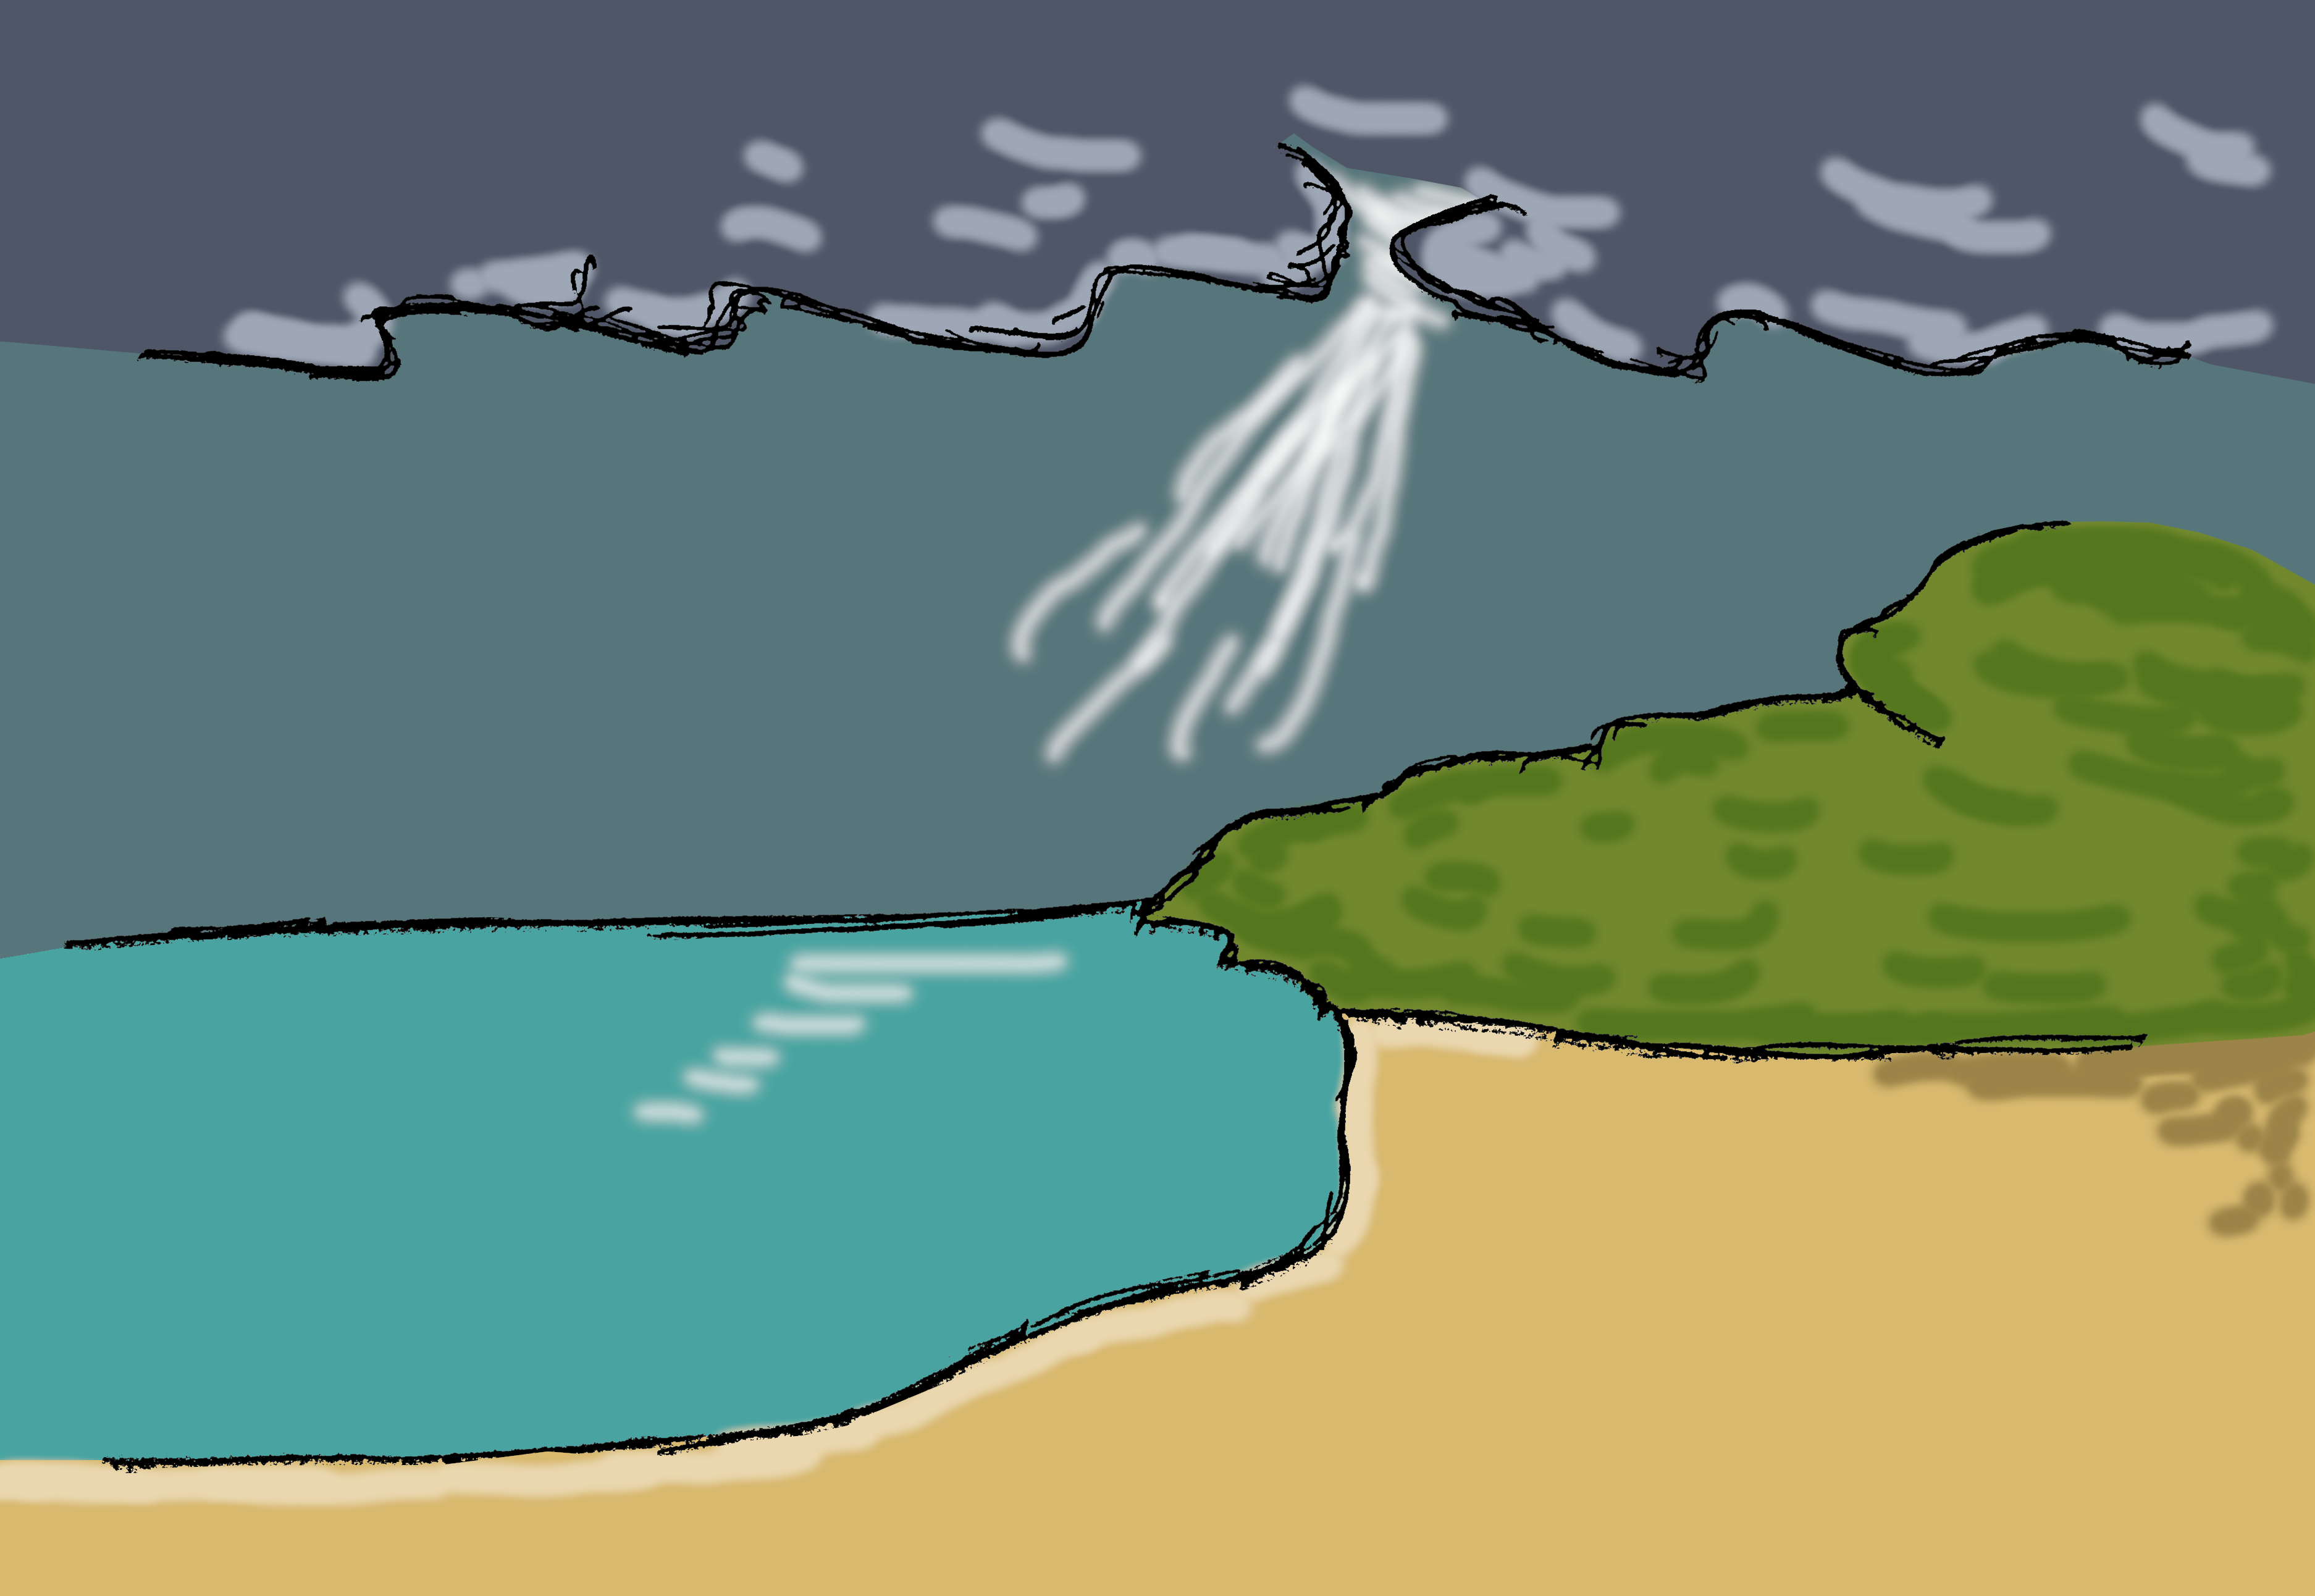
\includegraphics[width=26cm]{isola_principe}};
			\draw [ultra thick] (2,8) rectangle (28,-9);
			\draw [ultra thick, fill=dida] (1,14) rectangle (29,8);
			\node (example-textwidth-2) [right, align=left, text width=27cm, color=black, font=\fontsize{23pt}{24pt}\selectfont] at (1.5,11) {Era stata una mattinata nuvolosa, quella del 29 maggio del 1919 sull'Isola Principe, in Africa Occidentale. Finalmente verso mezzogiorno il cielo aveva iniziato ad aprirsi e la luce del Sole iniziava a filtrare tra le nubi. Il tempo, però, era tiranno e Arthur Eddington e Edwin Cottingham avevano le ore contate per fotografare l'eclissi solare totale che stava iniziando.};
		\end{scope}
		%eclipse
		\begin{scope}[shift={(0,-24)}]
			\draw [ultra thick, fill=space] (1.5,4.5) rectangle (28.5,-35.5);
			%dida
			\draw [ultra thick, fill=dida] (16.5,5.5) rectangle (29,-7.5);
			\node (example-textwidth-2) [right, align=left, text width=11.5cm, color=black, font=\fontsize{23pt}{24pt}\selectfont] at (17,-1) {Un'eclissi solare avviene quando la Luna si frappone tra la Terra e il Sole, bloccandone i raggi. Un evento di questo genere era anche quello perfetto per verificare una delle predizioni fatte dalla teoria della relatività generale di Einstein: la massa del Sole deformando lo spazio tempo costringe la luce a muoversi lungo un percorso curvo.};
			%
			\draw [ultra thick, fill=red] (2.5,-26) rectangle (10,-28);
			\node (example-textwidth-2) [right, align=left, text width=7cm, color=black, font=\fontsize{23pt}{24pt}\selectfont] at (3,-27) {Lo schema non è in scala};
			% sun
			\tkzDefPoint(8,-2){S}
			\tkzDefPoint(14,-2){S1}
			\tkzDefPoint(2,-2){S2}
			% earth
			\tkzDefPoint(24,-30){E}
			\tkzDefPoint(29,-30){E1}
			% moon
			\tkzDefBarycentricPoint(S=1,E=1.3) \tkzGetPoint{L}
			\tkzInterLC[R](S,E)(L,2 cm) \tkzGetPoints{C}{L1}
			%
			\tkzInterLC(L,E)(E,E1) \tkzGetPoints{e1}{e2}
			%
			\tkzTangent[from=e1](L,C) \tkzGetPoints{l1}{l2}
			\tkzTangent[from=e1](S,S1) \tkzGetPoints{s1}{s2}
			\tkzTangent[from=l1](E,E1) \tkzGetPoints{ea}{eb}
			\tkzTangent[from=l2](E,E1) \tkzGetPoints{ec}{ed}
			%
			\tkzDrawSegments[color=white,ultra thick](e1,s1 e1,s2)
			\tkzDrawSegments[color=white,ultra thick](l1,eb l1,s2)
			\tkzDrawSegments[color=white,ultra thick](l2,ec l2,s1)
			%
			\tkzDrawPolygon[fill=white,opacity=0.5](s1,s2,e1)
			\tkzDrawPolygon[fill=moon,opacity=0.5](l1,l2,ec,eb)
			%
			\tkzDrawCircle[fill=moon](L,C)
			\tkzDrawCircle[fill=earth](E,E1)
			\tkzDrawCircle[fill=white](S,S1)
			%
		\end{scope}
		%
		\begin{scope}[shift={(0,-63)}]
			\draw [ultra thick, fill=space] (1,2.5) rectangle (29,-15);
			\tkzDefPoint(28,-1.5){S1}
			\tkzDefPoint(27.5,-1.5){Sr1}
			\tkzDefPoint(28,-10){S2}
			\tkzDefPoint(27.5,-10){Sr2}
			\tkzDefPoint(15.3,-4.95){I}
			%
			\tkzDefPoint(3,-8){E}
			\tkzDefPoint(1.5,-8){Er}
			%
			\tkzDefPoint(15,-9){S}
			\tkzDefPoint(12,-9){Sr}
			%
			\tkzDrawSegment[color=white, ultra thick](E,S1)
			\tkzDrawSegment[color=white, ultra thick](I,S2)
			\draw (15,-5.2) [color=white, ultra thick, partial ellipse=53:100:0.5 and 0.3];
			\tkzDrawCircle[fill=earth](E,Er)
			\tkzDrawCircle[fill=white](S1,Sr1)
			\tkzDrawCircle[fill=white](S2,Sr2)
			\tkzDrawCircle[fill=white](S,Sr)
			%
			\draw [ultra thick, fill=red] (25.3,-2.5) rectangle (30,-4.5);
			\node at (25.5,-3.5) (example-textwidth-2) [right, align=left, text width=5cm, color=black, font=\fontsize{23pt}{24pt}\selectfont] {Posizione apparente};
			%
			\draw [ultra thick, fill=red] (25.3,-11) rectangle (30,-13);
			\node at (25.5,-12) (example-textwidth-2) [right, align=left, text width=5cm, color=black, font=\fontsize{23pt}{24pt}\selectfont] {Posizione reale};
			%
			\draw [ultra thick, fill=dida] (2.5,5) rectangle (20.5,-1);
			\node (example-textwidth-2) [right, align=left, text width=17cm, color=black, font=\fontsize{23pt}{24pt}\selectfont] at (3,2) {Dopo aver scattato 16 fotografie Eddington e gli altri suoi colleghi andati in Brasile, a Sobral, tornati in patria, fanno i conti e mostrano che Einstein aveva ragione: la luce intorno al Sole segue un percorso curvo!};
		\end{scope}
		%
		\begin{scope}[shift={(0,-87)}]
			\draw [ultra thick, fill=space] (-1,8) rectangle (31,-8);
			\node at (24,0) {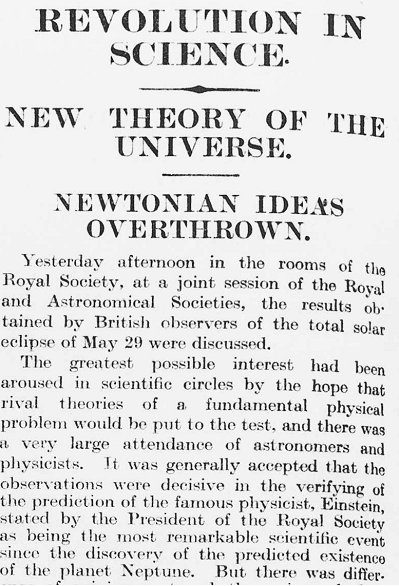
\includegraphics[width=10cm]{relativity_eddington_times}};
			\draw [ultra thick, fill=dida] (0.5,10) rectangle (18.5,4);
			\node (example-textwidth-2) [right, align=left, text width=17cm, color=black, font=\fontsize{23pt}{24pt}\selectfont] at (1,7) {La notizia venne diffusa il 7 novembre del 1919 sulle pagine del Times di Londra, giusto il giorno dopo l'annuncio scientifico fatto durante il congresso della Royal Society: \textbf{Albert Einstein aveva ragione}!};
		\end{scope}
		%
		\begin{scope}[shift={(0,-96)}]
			\node at (27,0) () {
\includegraphics[width=3.7cm]{licenza}};
			\node at (18,-0.1) {\textcolor{black}{\fontsize{14}{15}\selectfont Testo e illustrazioni: @ulaulaman - Gianluigi Filippelli}};
		\end{scope}
	\end{tikzpicture}
%
\end{document}